%!BIB program=biber
\documentclass[scheme=chinese,a4paper]{article}
\usepackage[utf8]{inputenc}
\usepackage{amsmath}
\usepackage{esint}
\usepackage{tabstackengine}
\usepackage{xeCJK}
\usepackage{caption} 
\usepackage{stackengine}
\usepackage{graphicx}
\graphicspath{ {../resources/figure/sensor/} }
\usepackage{float}
\usepackage{amsmath}
\usepackage{ulem}
\usepackage{amsfonts}
\usepackage{xcolor}
\usepackage{tikz}
\usetikzlibrary{calc}
\usepackage{pgfplots}
\usepackage{mathrsfs}
\usepackage{listings}
\lstset{basicstyle=\ttfamily\footnotesize,breaklines=true}
\usepackage{url}
\usepackage[colorlinks,linkcolor=blue]{hyperref}
\usepackage{subcaption}
\usepackage{pdfpages}
\usepackage{svg}

% 修改列表的间距
\usepackage{enumitem}
\setlist[1]{itemsep=-5pt}

\usepackage[backend=biber,style=gb7714-2015]{biblatex} 
\addbibresource{../resources/bibs/refs.bib}

\usetikzlibrary{shapes,arrows}
\usetikzlibrary{arrows}

%%%% 下面的命令重定义页面边距,使其符合中文刊物习惯 %%%%
\addtolength{\topmargin}{-54pt}
\setlength{\oddsidemargin}{0.63cm}  % 3.17cm - 1 inch
\setlength{\evensidemargin}{\oddsidemargin}
\setlength{\textwidth}{14.66cm}
\setlength{\textheight}{24.00cm}    % 24.62

%%%% 段落首行缩进两个字 %%%%
\makeatletter
\let\@afterindentfalse\@afterindenttrue
\@afterindenttrue
\makeatother

\setlength{\parindent}{1em}  %中文缩进一个汉字位

%%%% 下面的命令设置行间距与段落间距 %%%%
\linespread{1.4}

%段间距等于行间距
\setlength{\parskip}{0pt}

%%%% 重定义 %%%%
\renewcommand{\contentsname}{目录}  % 将Contents改为目录
\renewcommand{\abstractname}{摘要}  % 将Abstract改为摘要
\renewcommand{\refname}{参考文献}   % 将References改为参考文献
\renewcommand{\indexname}{索引}
\renewcommand{\figurename}{图}
\renewcommand{\tablename}{表}
\renewcommand{\appendixname}{附录}
% \renewcommand{\algorithm}{算法}
\title{基于LoRaWAN的智慧农业方案}
\author{莫健}
\date{2021 五月}


\begin{document}
\maketitle
\begin{abstract}
  本文简单介绍了LoRa以及LoRaWAN的特性以及应用场景, 阐述了LoRaWAN相对于其他协议的优越之处, 并提出了一种利用Arduino和Raspberry Pi, 借由Chirpstack网关平台以及各类传感器搭建的可能的LoraWAN在智慧农业中的应用方案. 
\end{abstract}
\tableofcontents
\newpage
\section{背景介绍}
我国是农业大国, 农业经济将长期在国民经济中处于重要地位。但现今我国大部分地区还维持着传统农业粗放的管理方式,凭借经验施肥灌溉,不仅需要大量的人力物力,对环境保护以及水土保持构成严重威胁,还因无法对农业环境信息实现精细化、智能化管理,影响了农业的可持续发展。

\subsection{智慧农业应用场景}
随着中国经济的快速增长,人们的生活水平也在不断提高,蔬菜作为日常生活的必需品,消费者对于蔬菜的产量和品质要求也变得越来越高。通过应用智慧温室大棚来种植蔬菜,可以对蔬菜生长过程中的各个环节都进行科学的把控,从而不断提升蔬菜的产量和质量,进一步满足市场中消费者的需求。\cite{lorawan_2}
\begin{itemize}
  \item\textbf{牲畜管理 }农民可以更好地监测动物状况,如体温、发情、疾病、生产力、位置,以及更好地防止牲畜的丢失或被盗。
  \item\textbf{环境监测 }农民可以准确地记录降雨和其他天气状况,在水质变化或过度使用植物检疫产品时设置洪水风险警报和其他警报。
  \item\textbf{资产管理 }农民现在可以监督仓储条件,收到关于闸门和设备的警报,更好地跟踪和控制整个供应链。
  \item\textbf{灌溉控制 }农民现在可以安排并将适量的水用于农作物,减少浪费和成本。
  \item\textbf{土壤健康 }农民可以监测从表面到根部的土壤质量,比较区域,调节施肥,分析历史模式,更好地长期管理作物。
\end{itemize}



\section{通信协议}
\subsection{LPWAN}
LPWAN(Low-Power Wide-Area Network,低功率广域网络)也称为LPWA (Low-Power Wide-Area) ,或 LPN(Low-Power Network,低功率网络),是一种用在物联网(例如以电池为电源的传感器),可以用低比特率进行长距离通讯的无线网络。

\paragraph{优点}LPWAN\cite{wiki:LPWAN}可以用来建立一个私有的无线感测网络,但也可以是一个第三方提供的服务或基础设施,这使传感器的拥有者可以直接部署传感器,而不必投资经费于网关的建设。LPWAN是某些需要定期或不一致的数据长期远距离传输的用例的绝佳解决方案。想想智能垃圾处理仪、智能停车仪或土壤和水质传感器。
\paragraph{缺点}LPWAN不适合需要频繁和/或大量传输数据的用例。LPWANs通常携带300 bit/s到50 kbit/s的数据包。还记得56 kbit/s或 拨号上网吗?通过拨号传输的数据比大多数数据密集型的LPWAN要多,所以你不会在大多数LPWAN上发送猫的照片、小狗的视频或漫无边际的语音邮件。这不是它们的目的。

LoRa和LoRaWAN属于非蜂窝式LPWAN无线通信网络协议和参与者,在免许可频段运行。其他在免许可频段运行的技术包括Sigfox、Ingenu。
\subsection{LoRa}
LoRa使用线性调频扩频调制技术,即保持了像FSK(频移键控)调制相同的低功耗特性,又明显地增加了通信距离,同时提高了网络效率并消除了干扰,即不同扩频序列的终端即使使用相同的频率同时发送也不会相互干扰。

线性扩频已在军事和空间通信领域使用了数十年,因为其可以实现长通信距离和干扰的鲁棒性,而LoRa是第一个用于商业用途的低成本实现。随着LoRa的引入,嵌入式无线通信领域的局面发生了彻底的改变。这一技术改变了以往关于传输距离与功耗的折衷考虑方式,提供一种简单的能实现远距离、长电池寿命、大容量、低成本的通讯系统。
\subsubsection{扩频因子}
LoRa是一种啁啾扩频调制方式。传输的数据,也就是一个符号,将由一个频率范围从$f_{min}$到$f_{max}$的啁啾信号来表示。在LoRa调制中,我们可以通过改变扩频因子和带宽参数来配置符号。一个符号需要$T_S$秒的时间来传输,这是带宽和扩频因子的函数,可以用下面的公式表示。
\begin{equation}
  T_S=\frac{2^{SF}}{BW}
\end{equation}

扩频因子(SF)决定了每秒发送多少个啁啾\footnote{在此啁啾(chirp)约等于码片(chip)},即数据的载体。网络根据通信设备和网关之间的环境条件来决定扩频因子(在7-12之间分级)。这假定自适应数据速率功能被打开,除了连续移动的设备外,建议所有的设备都这样做。

较低的SF意味着每秒发送更多的啁啾,因此,你可以每秒编码更多的数据。较高的SF意味着每秒钟发送较少的啁啾;因此,每秒钟要编码的数据较少。与较低的SF相比,用较高的SF发送相同数量的数据需要更多的传输时间,即所谓的通话时间(airtime)。更多的通话时间意味着调制解调器启动和运行的时间更长,消耗的能量更多。

高SF的好处是,更多延长的通话时间使接收器有更多机会对信号功率进行采样,从而使灵敏度更高。更好的灵敏度意味着你可以在更远的地方接收信号,所以你可以得到更好的覆盖。理论上,SF每提高一个档次,传输相同数量的数据的时间就增加一倍。
\subsubsection{编码率}
LoRa调制还在每次数据传输中增加了前向纠错编码(FEC)。这种实现方式是将带有冗余的4位数据编码为5位、6位、7位、甚至8位。使用这种冗余将使LoRa信号能够经受住短时干扰。编码率(CR)值需要根据用于数据传输的信道条件来调整。如果信道中的干扰太多,那么建议增加CR值。然而,CR值的增加也会增加传输的时间。

CR值越大,则实际一个符号中的有效数据更少,所以速率也就更低,但是鲁棒性会更好。
\subsubsection{LoRa 物理帧}
\begin{figure}[H]
\centering
\includegraphics[width=0.7\textwidth]{lora_phy_frame.png}
\caption{LoRa物理帧\cite{lora_unknown}}
\end{figure}
\begin{figure}[H]
\centering
\includegraphics[width=0.9\textwidth]{Lora_sym.png}
\caption{LoRa 物理帧的频谱图\cite{lora_study}}
\end{figure}
\begin{itemize}
  \item\textbf{Preamble}用于保持接收机与输入的数据流同步。默认是12个符号长度,LoRaWAN中使用8个符号长度。前导长度是一个可以通过编程来设置的变量,所以前导码的长度可以扩展。接收机的前导码长度应与发射机一致。如果前导码长度为未知或可能会发生变化,应将接收机的前导码长度设置为最大值。可以通过设置前导码值进行地址过滤,实现分组通信。
  \item\textbf{Header}包含的信息有,Payload的字节数、编码率、是否打开Payload CRC。
  \item\textbf{Payload}真正发送的数据
  \item\textbf{Payload CRC}对Payload的CRC校验
\end{itemize}



\subsection{LoRaWAN}
LoRa是用于长距离、低功率通信链接的物理层或调制技术。LoRaWAN是一种通信协议和网络架构,位于LoRa物理层之上。
\begin{figure}[H]
  \centering
  \includegraphics[width=0.9\textwidth]{LA_System_0.png}
  \caption{LoRaWAN 流图}
  \end{figure}
LoRaWAN 网络通常采用星型拓扑结构,其中网关(gateway)转发终端设备(end-devices)和中心网络服务器(Network Server)之间的消息,而网络服务器将来自网络的每个设备的数据包发送到关联的应用服务器(Application Server)。为了保证无线射频传输的安全,LoRaWAN 协议采用对称加密方法,这种方法使用会话密钥(从设备的根密钥计算得到)。在后端,设备的根密钥的存储和相关的密钥计算操作由入网服务器(Join Server)保证。
\begin{figure}[H]
\centering
\includegraphics[width=0.9\textwidth]{lorawan.png}
\caption{LoRaWAN 协议栈}
\end{figure}

% 一点对多点通信,多个从节点可同时与中心点通信,从节点可随机上报数据,节点可以根据外界环境和信道阻塞自动采取跳频和速率自适应技术,逻辑上网关可以接收不同速率和不同频点的信号组合,物理上网关可以同时接收8路、16路、32路甚至更多路数据,减少了大量节点上行时冲突的概率。
% \begin{figure}[H]
% \centering
% \includegraphics[width=0.5\textwidth]{mesh_star.jpeg}
% \caption{Mesh组网和星形组网}
% \end{figure}
LoraWAN 具有以下特点
\begin{itemize}
  \item 远距离 (城市大于5公里, 郊区大于10公里)
  \item 低成本 (每模块低于5美元)
  \item 双向通信
  \item 安全, 经过加密
  \item 在非授权频谱中运行
  \item 低比特率(0.3 bps - 50 kbps,通常约为10 kB/天
\end{itemize}
\subsubsection{速率自适应机制}
为了最大程度地延长终端的电池寿命和扩大网络容量,LoRaWAN 网络设施使用速率自适应(adaptive data rate,ADR)机制来独立管理每个终端的速率和RF输出。ADR机制控制终端设备的以下传输参数。
\begin{itemize}
  \item 扩频因子
  \item 带宽
  \item 传输功率
\end{itemize}
ADR可以优化设备的功耗,同时确保在网关处仍能收到信息。当ADR使用时,网络服务器将向终端设备指示它应该降低传输功率或提高数据速率。靠近网关的终端设备应使用较低的扩频因子和较高的数据速率,而较远的设备应使用高扩频因子,因为它们需要较高的链路预算。

ADR算法不适用于移动终端,若终端节点位置相对于网关位置经常发生改变,那么基于最近数据包信号质量而选择的数据速率可能会和新环境不匹配而导致通信丢包。

但目前LPWAN行业的典型应用基本都是静态节点,如水电表、地磁、门锁、温湿度之类,对于这些静态终端以及部分偶尔发生移动的终端设备,ADR功能都可以有效地将通信速率调节至合理,并且对于偶发的位置变化导致的数据丢包也可以在一定时间内进行自愈。
\subsubsection{入网方式}
\begin{figure}[H]
\centering
\includegraphics[width=0.8\textwidth]{lorawan_frame.jpg}
\caption{LoraWAN 帧格式}
\end{figure}
\paragraph{OTAA}
OTAA(Over-The-Air Activation)入网方式的节点需要发送一条Join Request入网请求,然后接收到NS下发的Join Accept入网应答之后,从入网应答中解析出DevAddr、NwkSKey和AppSKey之后,才是入网成功。因为节点需要使用这三个参数对所发的数据进行加密以保证数据的安全性。

OTAA 需要以下参数以成功入网
\begin{itemize}
  \item DevEUI - 64位终端设备标识符,EUI-64(唯一)
  \item DevAddr - 32位设备地址(非唯一)
  \item AppEUI - 64位应用标识符,EUI-64(唯一)
  \item GatewayEUI - 64位网关标识符,EUI-64(唯一)
\end{itemize}

OTAA终端在弱网区域的表现能力相对较差。在弱网区域,虽然网关有可能接收到终端发送的Join Request入网请求,但是通过网关转发的Join Accept请求,因为信号质量的问题,终端却不一定能接收到。OTAA终端无法入网的情况下,就无法获取到三个加密参数,导致OTAA终端无法工作。
\paragraph{ABP}
 ABP(Activation by Personalization)在某些特定场景下是比OTAA更有优势的。弱网区域,顾名思义就是网络覆盖信号较差的区域。比如网络覆盖的边缘区域,或者一些障碍物较多,还有一些其他严重影响网络信号的区域。

在LoRaWAN网络中,网关的接收能力是要大于终端的接收能力的。在弱网区域,网关还有可能接收到终端发送的数据,但是终端不一定能够接收到网关发送的数据。

而ABP终端在弱网区域的表现能力是强于OTAA终端的,因为ABP终端不需要执行入网操作,它可以不需要服务器给它下发任何消息。ABP终端配置了三个加密参数,所以ABP终端可以直接工作。
\subsubsection{终端}
入网之后,应用数据就被加密处理了。LoRaWAN规定数据帧类型有 Confirmed 或者 Unconfirmed 两种,即「需要应答」 和「不需要应答」类型。厂商可以根据应用需要选择合适的类型。

LoRaWAN设计之初的一大考虑就是要支持应用多样性。除了利用 AppEUI 来划分应用外,在传输时也可以利用 FPort 应用端口来对数据分别处理。FPort 的取值范围是(1$\sim$223),由应用层来指定。

每个设备可以在任意可用的信道,任意时间,使用任意可用数据速率发送数据,只要遵守如下规定
\begin{itemize}
  \item 终端的每次传输都使用伪随机方式来改变信道。频率的多变使得系统具有更强的抗干扰能力。
  \item 终端要遵守相应频段和本地区的无线电规定中的最大发射占空比要求。
  \item 终端要遵守相应频段和本地区的无线电规定中的最大发射时长(或驻留时间)要求。
\end{itemize}
LoraWAN 对终端设备分为三类
\begin{figure}[H]
\centering
\includegraphics[width=0.7\textwidth]{lorawan_device.png}
\caption{LoraWAN 设备分类}
\end{figure}
\paragraph{Class A}
Class A 的终端在每次上行后都会紧跟两个短暂的下行接收窗口,以此实现双向传输。终端基于自身通信需求来安排传输时隙,在随机时间的基础上具有较小的变化(即ALOHA协议)。这种 Class A 操作为应用提供了最低功耗的终端系统,只要求应用在终端上行传输后的很短时间内进行服务器的下行传输。服务器在其他任何时间进行的下行传输都得等终端的下一次上行。
\begin{figure}[H]
\centering
\includegraphics[width=0.6\textwidth]{class_a.png}
\caption{Class A 上下行时序图}
\end{figure}
\paragraph{Class B}
Class B 的终端会有更多的接收时隙。除了 Class A 的随机接收窗口,Class B 设备还会在指定时间打开别的接收窗口。为了让终端可以在指定时间打开接收窗口,终端需要从网关接收时间同步的信标(Beacon)。
\begin{figure}[H]
\centering
\includegraphics[width=0.8\textwidth]{class_b.png}
\caption{Class B 上下行时序图}
\end{figure}
\paragraph{Class C}
Class C 的终端基本是一直打开着接收窗口,只在发送时短暂关闭。Class C 的终端会比 Class A 和 Class B 更加耗电,但它们从服务器到终端下行的通信时延也是最短的。
\begin{figure}[H]
\centering
\includegraphics[width=0.8\textwidth]{class_c.png}
\caption{Class C 上下行时序图}
\end{figure}

\subsubsection{网关}
网关是建设LoRaWAN网络的关键设备,目的是缓解海量节点数据上报所引发的并发冲突。
网关通过可靠的标准 IP 连接来接入网络服务器,终端则通过单跳的 LoRa 或者 FSK 来和一个或多个网关通讯。虽然主要传输方式是终端上行传输给网络服务器,但所有的传输通常都是双向的。
终端和网关间的通讯被分散到不同的信道(frequency channels)和数据速率(data rates)上。数据速率的选择需要权衡通信距离和消息时长两个因素,使用不同数据速率的设备互不影响。
\begin{itemize}
  \item 兼容性强,所有符合LoRaWAN协议的应用都可以接入
  \item 接入灵活,单网关可接入几十到几万个节点,节点随机入网,数目可延拓
  \item 并发性强,网关最少可支持8频点,同时随机8路数据并发,频点可扩展
  \item 可实现全双工通信,上下行并发不冲突,实效性强
  \item 灵敏度高,同速率下比非LoRaWAN设备的灵敏度更高
  \item 网络拓扑简单,星状网络可靠性更高,功耗更低
  \item 网络建设成本和运营成本很低。
\end{itemize}
\subsection{其他通信协议}
\subsubsection{ZigBee}
ZigBee是一个Mesh网状网络,因此ZigBee系统中的每个节点都可以作为一个无线数据终端或中继器。数据从一个节点到另一个节点,直到到达路由器。它是为相对较低的数据速率应用而设计的,它经常被用于家庭自动化和智能照明。
\subsubsection{NB-IoT}
基于蜂窝的窄带物联网(Narrow Band Internet of Things,NB-IoT)是万物互联网络的一个重要分支。NB-IoT构建于蜂窝网络,只消耗大约180KHz的带宽,可直接部署于GSM网络、UMTS网络或LTE网络,以降低部署成本、实现平滑升级。

NB-IoT是IoT领域一个新兴的技术,支持低功耗设备在广域网的蜂窝数据连接,也被叫作低功耗广域网(LPWAN)。NB-IoT支持待机时间长、对网络连接要求较高设备的高效连接。据说NB-IoT设备电池寿命可以提高至至少10年,同时还能提供非常全面的室内蜂窝数据连接覆盖。
\section{硬件选型}
\subsection{Arduino}
Arduino电路板设计使用各种微处理器和控制器。\cite{wiki:Arduino}这些电路板配有一组数字和模拟I/O引脚,可以连接各种扩展板或面包板(屏蔽板)和其他电路。这些电路板具有串行通信接口,包括某些型号上的通用串行总线(USB),也用于从个人电脑加载程序。微控制器通常使用C/C++编程语言。除了使用传统的编译工具链之外,Arduino项目还提供了一个基于Processing语言项目的集成开发环境。Arduino允许任何人制造Arduino板和软件分发。 Arduino板可以以预装的形式商业销售,也可以作为DIY包购买。

\begin{figure}[H]
  \begin{subfigure}[t]{0.25\textwidth}
    \includegraphics[width=\textwidth]{arduino_uno.jpg}
    \caption{Arduino UNO}
  \end{subfigure}
  \begin{subfigure}[t]{0.45\textwidth}
    \includegraphics[width=\textwidth]{arduino_mega.jpg}
    \caption{Arduino MEGA}
  \end{subfigure}
  \begin{subfigure}[t]{0.25\textwidth}
    \includegraphics[width=\textwidth]{arduino_nano.jpg}
    \caption{Arduino NANO}
  \end{subfigure}
  \caption{Arduino 官方开发板}
\end{figure}

Arduino Core 提供了低级别的API(Application Programming Interface),这些API在Arduino参考页中有记录。例如\lstinline{digitalRead, digitalWrite, delay}等等。核心文件通常包含Atmel公司的\lstinline{include}文件,这些文件为芯片中的各种寄存器提供了文件化的名称。

\begin{figure}[H]
  \begin{subfigure}[t]{0.25\textwidth}
    \includegraphics[width=\textwidth]{ESP3.png}
    \caption{ESP32}
  \end{subfigure}
  \begin{subfigure}[t]{0.45\textwidth}
    \includegraphics[width=\textwidth]{stm_2.jpg}
    \caption{STM32 Nucleo-64}
  \end{subfigure}
  \begin{subfigure}[t]{0.25\textwidth}
    \includegraphics[width=\textwidth]{Seed.jpg}
    \caption{Seeeduino Xiao}
  \end{subfigure}
  \caption{Arduino 兼容开发板}
\end{figure}
由于每种芯片类型都有不同的寄存器地址,所以你需要为每种处理器芯片提供不同的内核。此外,在某些情况下,人们将芯片组装到不同的板子上,Core 将反映板子的接线方式。例如,一块板子上的 "PIN 8"与另一块板子相比,可能连接到处理器芯片上的不同针脚。因此,如果你从第三方购买电路板,他们也可能提供他们自己的核心文件。
\subsection{Raspberry Pi}
树莓派(Raspberry Pi)是尺寸仅有信用卡大小的一个小型电脑。\cite{wiki:raspberry_pi}与常见的51单片机和STM32等这类的嵌入式微控制器相比,不仅可以完成相同的IO引脚控制之外,还能运行有相应的操作系统,可以完成更复杂的任务管理与调度,能够支持更上层应用的开发,为了开发者提供了更广阔的应用空间。比如开发语言的选择不仅仅只限于C语言,连接底层硬件与上层应用,可以实现物联网的云控制和云管理,也可以忽略树莓派的IO控制,使用树莓派搭建小型的网络服务器,做一些小型的测试开发和服务。
\begin{figure}[H]
  \begin{subfigure}[t]{0.33\textwidth}
    \includegraphics[width=\textwidth]{rasp_4.jpg}
    \caption{树莓派4}
  \end{subfigure}
  \begin{subfigure}[t]{0.33\textwidth}
    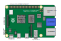
\includegraphics[width=\textwidth]{RaspberryPi_Model_4B.png}
    \caption{树莓派4引脚图}
  \end{subfigure}
  \begin{subfigure}[t]{0.3\textwidth}
    \includegraphics[width=\textwidth]{RASP_PI_ZERO.png}
    \caption{树莓派 Zero}
  \end{subfigure}
  \caption{树莓派官方开发板}
\end{figure}
Armbian是一个用于单板计算机(single board computers)的基础操作系统平台,其他项目可以基于它来构建。具有以下特点
\begin{itemize}
  \item 基于Debian或Ubuntu的轻量级Linux分布,专门用于ARM开发板
  \item 每个系统都由Armbian构建工具进行编译、组装和优化
  \item 它拥有强大的构建和软件开发工具,可以进行自定义构建
  \item 一个充满活力的社区
\end{itemize}

\subsection{RAK2245 RPi HAT}
\begin{figure}[H]
\centering
\includegraphics[width=0.33\textwidth]{rak2245.png}
\caption{RAK2245}
\end{figure}
RAK2245 Pi HAT是一个具有Raspberry PI外形的模块。它可以插入Raspberry PI,如Raspberry Pi 3 Model B+,作为网关的一个完整的射频前端。它支持八个频道,可用于LoRaWAN全球频段。该板是最小的网关集中器,集成了Ublox MAX-7Q GPS模块和散热器。
\begin{figure}[H]
\centering
\includegraphics[width=0.9\textwidth]{rak2245-pihat-block-diagram.png}
\caption{RAK2245系统框图}
\end{figure}
该板能以超快的速度提供低数据率的LoRa无线链接。它由一个Semtech SX1301收发器集中器供电,能够管理来自许多远程分散的终端的数据包。两个Semtech SX125X被整合为射频前端I/Q收发器。
\subsection{RAK811}
\begin{figure}[H]
  \begin{subfigure}[t]{0.33\textwidth}
    \includegraphics[width=\textwidth]{rak811_wisnode.png}
    \caption{Arduino 扩展版}
  \end{subfigure}
  \begin{subfigure}[t]{0.33\textwidth}
    \includegraphics[width=\textwidth]{RAK811.png}
    \caption{RAK811 封装}
  \end{subfigure}
  \begin{subfigure}[t]{0.33\textwidth}
    \includegraphics[width=\textwidth]{RAK811J_2.png}
    \caption{RAK811 内部结构}
  \end{subfigure}
\caption{RAK811}
\end{figure}
RAK811 远距离LoRa 收发模块, 其拥有小巧、简单、远距离传输和低功耗的特点, LoRaWAN 组网方式, 该模块集成了Semtech SX1276芯片, 依靠内置的STM32L 芯片提供UART接口, 能够通过简单的AT串口指令来进行LoRa模块的配置与数据收发. 

“Shields”扩展版能够被插入Arduino和Arduino兼容硬件。用途是增加Arduino硬件上没有的功能,如马达控制、GPS、有线网络、液晶显示器或者是面包板。
\subsection{DHT11 数字温湿度传感器}
\begin{figure}[H]
\centering
\includegraphics[width=0.33\textwidth]{DHT11.jpg}
\caption{DHT11}
\end{figure}
DHT11数字温湿度传感器是一款含有已校准数字信号输出的温湿度复合传感器。它应用专用的数字模块采集技术和温湿度传感技术,确保产品具有极高的可靠性与卓越的长期稳定性。传感器包括一个电阻式感湿元件和一个NTC测温元件,并与一个高性能8位单片机相连接。因此该产品具有品质卓越、超快响应、抗干扰能力强、性价比极高等优点。
\subsection{LM35温度传感器}
\begin{figure}[H]
\centering
\includegraphics[width=0.33\textwidth]{LM35.jpg}
\caption{LM35}
\end{figure}
基于LM35半导体的温度传感器,可以用来对环境温度进行定性的检测。LM35半导体温度传感器是美国国家半导体公司生产的线性温度传感器。其测温范围是-40℃到150℃,灵敏度为10mV/℃,输出电压与温度成正比。温度测量常用的传感器包括热电偶,铂电阻,热敏电阻和半导体测温芯片,其中热电偶常用于高温测量,铂电阻用于中温测量(到摄氏800度左右),而热敏电阻和半导体温度传感器适合于100-200度以下的温度测量,其中半导体温度传感器的应用简单,有较好的线性度和较高的灵敏度。
\subsection{TSL25911 光传感器模块}
\begin{figure}[H]
\centering
\includegraphics[width=0.33\textwidth]{TSL25911.jpg}
\caption{TSL25911}
\end{figure}
本产品采用TSL25911FN为核心,是一款基于IIC总线通信的光强数字转换器。传感器将一个宽带光电二极管(可见光和红外光)和一个红外响应光电二极管组合在能够在有效的16 位动态范围(16 位分辨率)上提供近光适应响应的单个 CMOS 集成电路上。两个积分 ADC将光电二极管电流转换为表示在每个通道上测量的辐照度的数字输出。该数字输出可以被输到微处理器,其中使用经验公式导出以勒克斯为单位的照度(环境光水平)以近似人眼反应。
\section{系统设计}
农田环境监测系统的设计, 要实现对农田土壤情况和气象环境参数进行有效的监测。系统设计要对每个农作物的节点进行实时的数据监测, 包括生长情况、湿度和水质等基本的环境参数。系统数据处理流程是要把每个监测点的参数数据及时地反馈给网络中继, 然后网络中继再把数据信息发给系统的数据中心, 存入数据库中由数据中心对数据进行科学分析。在客户端采用Web技术对系统数据库中的数据进行查询, 在Web 界面把数据展示给用户, 这样用户只要通过PC 和手机移动终端就可以对农作物的监测数据进行查看。
\subsection{感知层}
系统感知层是整个系统最基础且最重要的部分, 由各个传感器采集节点组成, 各传感器节点被放在不同的区域, 用来采集环境信息, 并将数据传输到应用层, 以供用户进行管理. \cite{lorawan_1}
\begin{figure}[H]
\centering
\includegraphics[width=0.8\textwidth]{end_device.jpg}
\caption{终端系统运行流程图}
\end{figure}
农作物生长环境比较复杂, 监测系统设计要满足可以实现长期稳定的数据监测, 系统中的传感器节点的安装要可以防范恶劣的天气和环境对其造成的影响。系统对传感器的设计, 要保证可以对监测对象进行准确的定位, 对农作物种植和生长的重要参数要进行实时监测。传感器在设计的时候要采用电池供电的方式, 并实现对数据的传输自动化和智能化。这样可以保证系统的稳定性, 以及对环境参数监测的准确性。
\subsection{应用层}
ChirpStack开源LoRaWAN网络服务器栈为LoRaWAN网络提供开源组件。它们共同构成了一个随时可用的解决方案,包括用于设备管理的用户友好型网络界面和用于集成的API。模块化的结构使其有可能整合到现有的基础设施中。所有组件都在MIT许可下授权,可用于商业目的。

利用任何兼容的编程语言均可实现一个MQTT客户端, 使用MQTT协议与ChirpStack网关服务器交互, 实现从网关发送与接收相应的数据. 

\section{结语}
根据农作物生产环境的具体需求对农田环境监测系统进行设计, 可以有效地提高农田环境监测的准确性和可靠性。基于LoRaWAN 物联网技术的农田环境监测系统的研究, 为建立完整的农田环境物联网监测系统提供了有效的依据, 不仅提高了农业生产的精准性, 而且促进了农业物联网的发展。基于LoRaWAN 技术设计的智慧农业系统方案还可应用于多种场合环境监测应用, 具有一定的应用前景, 希望能够为今后LoRaWAN 应用开发提供一定的参考借鉴.
\section{参考文献}
\printbibliography[heading=none]
\end{document}